\subsection{Dati e risultati}

\paragraph{Battito cardiaco}

Per capire come misurare l'attività cardiaca è necessaria una breve introduzione
al funzionamento del cuore. In cuore è composto da due atrii e due ventricoli,
come mostrato in figura \ref{fig:heart7}. Si gonfiano e si contraggono prima gli atrii e poi ventricoli
in modo da pompare il sangue lungo i vasi sanguigni. Un apposito sistema di valvole
fa in modo che il sangue non venga spinto nella direzione sbagliata diminuendo l'efficienza
dell'organo.

Ma come fa in cuore a coordinare con precisione le contrazioni? La membrana cellulare di tutte
le cellule del corpo, in condizioni normali, è polarizzata, ovvero c'è una differenza di potenziale
tra interno ed esterno a causa delle diverse concentrazioni di ioni. Il miocardio, il muscolo cardiaco,
contiene alcune cellule (formanti il miocardio specifico) che sono in grado di depolarizzarsi. Queste cellule
forniscono, ad intervalli circa regolari, l'impulso elettrico che fa contrarre il cuore.
Essendo il cuore un organo complicato la stimolazione elettrica deve essere precisa ed è composta
di varie fasi che agiscono su svariate parti del cuore in successione.

\begin{figure}
    \centering
	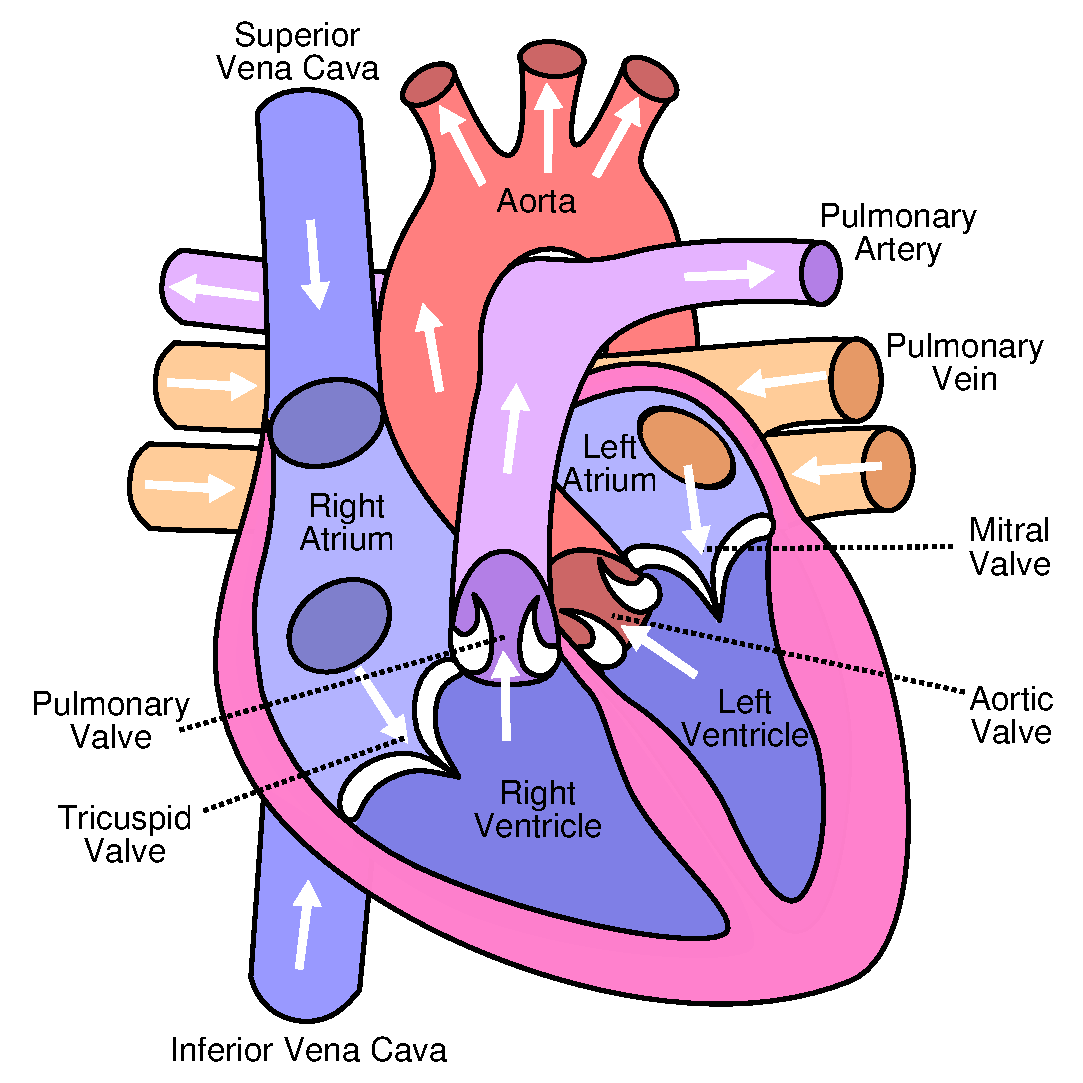
\includegraphics[width=\columnwidth]{figure/heart.pdf}
	\caption{}
	\label{fig:heart7}
\end{figure}

Poiché il corpo è un buon conduttore, essendo formato in gran parte da soluzioni ioniche, questi impulsi
si trasmettono facilmente a tutto il corpo, generando differenze di potenziale abbastanza semplici
da misurare. Così è possibile rilevare, senza interventi invasivi, le fasi di contrazione
del cuore e verificare l'insorgenza di problemi di salute.

\begin{figure}[b]
    \Large
    \begin{circuitikz}[scale=0.7, transform shape, inner sep=0.4mm]
        \foreach \y/\ytext in {0/,-4/'}
            \draw (0,\y)
            to [R=$R_T \ytext$,*-] ++(2,0) -- ++(1,0)
            to [battery, v=$E \ytext \simeq 700$ mV] ++(1.5,0)
            to [R=$R_1 \ytext$,-*] ++(2,0) -- ++(0,1)
            to [R=$R_2 \ytext$] ++(2,0) -- ++(0,-2)
            to [C=$C \ytext$] ++(-2,0) -- ++(0,1) ++ (2,0) node[circle=0.15cm, draw=black, fill=black]{} -- ++(1,0) node[circle=0.15cm, draw=black, fill=black]{};
        \draw[dashed] (2,1.5)--(2,-5.5);

        \node (sopra)  at ($(0,0)+(-0.2,-0.2)$)  {};
        \node (sotto)  at ($(0,-4)+(-0.2,+0.2)$) {};
        \draw [->] (sotto) to [out=135,in=225] node [left] {$\Delta V\ped{cuore}$} (sopra);
    \end{circuitikz}
    \caption{Le $R_T$ rappresentano la resistenza del corpo, mentre la parte a destra della
        linea tratteggiata é il circuito equivalente dell'elettrodo. }
    \label{fig:elettrodi7}
\end{figure}

Esistono decine di modi di disporre gli elettrodi sul corpo per misurare l'attività cardiaca e ognuna
porta a un diverso tipo di elettrocardiogramma. Il modo più semplice è usare 3 elettrodi: uno sulla caviglia
per mettere a comune il corpo, e due sui polsi per rilevare le differenze di potenziale generate dal miocardio
specifico (si può immaginare il miocardio come un momento di dipolo variabile che genera una differenza di potenziale).
Il nostro compito è di misurare, amplificare e filtrare queste minuscole differenze di potenziale
per poter leggere l'andamento temporale dell'attività cardiaca.

\begin{figure*}[b]
    \centering
	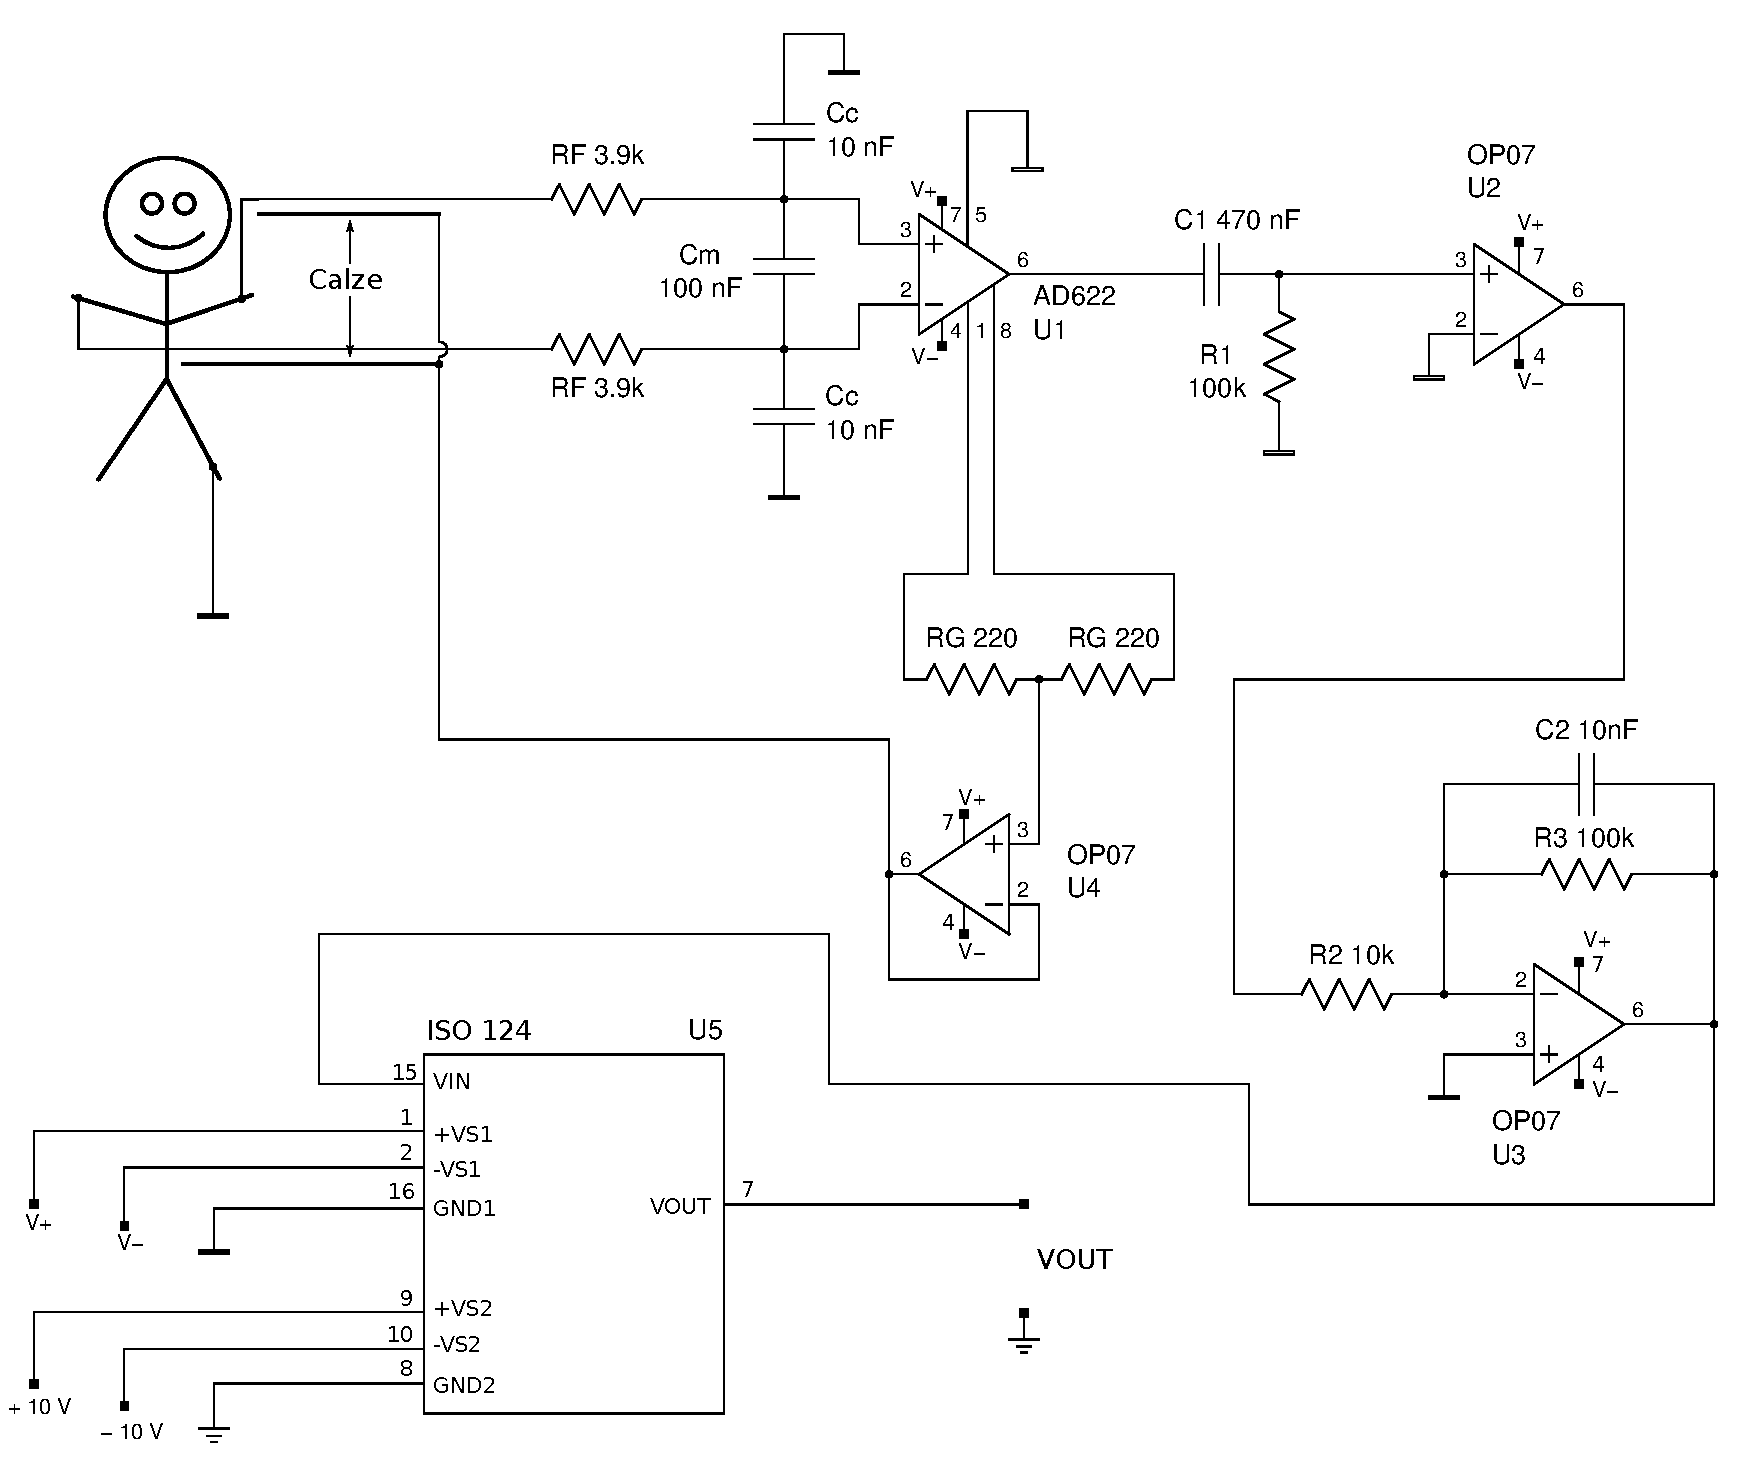
\includegraphics[width=0.9\textwidth]{figure/s.pdf}
	\caption{Circuito per la misura dell'ECG}
	\label{fig:circ7}
\end{figure*}

\paragraph{Difficoltà nella misura}

L'elettrocardiogramma è una misura piuttosto delicata, poiché ci sono molti fattori di disturbo, tra i quali:

\begin{itemize}
    \item{Movimenti e posizioni reciproche delle varie parti del corpo.}
    \item{Movimenti e posizioni dei cavi di collegamento.}
    \item{Interazioni tra corpo ed elettrodi. Il circuito \ref{fig:elettrodi7} mostra il circuito equivalente
        del sistema corpo + elettrodi.}
    \item{Effetti di induzione e capacitivi sulle varie parti del circuito e sul paziente dovuti per esempio
        alla tensione di rete.}
\end{itemize}

Tutti questi disturbi, uniti al fatto che il segnale elettrico proveniente dal cuore è di pochi
millivolt, rendono la misura difficoltosa. È quindi necessario prendere svariate precauzioni, che vedremo nel
prossimo paragrafo.

\paragraph{Blocchi funzionali}

Il circuito per la misura è mostrato in figura \ref{fig:circ7}. Il circuito è stato alimentato da due batterie da
9 V al fine di evitare contatti accidentali tra tensione di rete, terra e corpo. Questi contatti potrebbero portare
a folgorazioni del paziente. Analizziamo quindi i vari blocchi funzionali del circuito.

Il segnale che arriva dai polsi è piuttosto piccolo, nell'ordine dei millivolt, ed è molto sporco.
Il primo blocco è costituito da un amplificatore alle differenze AD622 il cui scopo è amplificare
la differenza di potenziale tra i polsi del paziente. Per ridurre il rumore i due ingressi sono dotati
di due filtri passa-basso formati dalle resistenze $R_F$ e dai condensatori $C_c$. Inoltre per ridurre
ulteriormente le frequenze molto alte, il condensatore $C_m$ mette gli ingressi in modo comune
a frequenze alte. Abbiamo poi scelto le resistenze di guadagno $R_G$ in modo da avere un guadagno elevato:
la scelta è caduta su due resistenze da \SI{220}{\ohm}, il guadagno dell'AD622 era quindi
$G = 1 + 2R_G/\SI{50.5}{\kilo\ohm} = 1 + 440/\SI{50.5}{\kilo\ohm} = 116$. 

Una volta amplificato il segnale, abbiamo utilizzato un filtro passa alto (blocco 2)
per eliminare le componenti continue e a bassa frequenza che a noi non interessano.
Questo filtro ha una capacità piuttosto grande per tagliare solo le componenti a bassissima frequenza
(ha una frequenza di taglio di circa 3-4 Hz), poiché il segnale cardiaco ha una frequenza di 1-2 Hz.
In questo modo, anche se il segnale viene attenuato un po', si eliminano le componenti continue e altri rumori
che non vogliamo avere nell'ECG. Il blocco contiene anche un follower (opamp U2),
per avere un alta impedenza all'uscita del filtro.

Infine il blocco 3 è costituito da un ulteriore stadio di amplificazione, realizzato con un operazionale in modalità
di amplificatore invertente con guadagno G = -10. L'unica cosa da notare è la capacità $C_2$, che non è altro che un ulteriore
filtro per il rumore ad alta frequenza. Il condensatore evita che vengano amplificato i segnali ad alte frequenze.

Un altro accorgimento per ridurre il rumore è il blocco 4. Questo blocco preleva tra le 2 $R_G$ la media
delle due tensioni all'ingresso dell'AD622 e dopo l'opamp U4, la cui funzione è solo di
aumentare l'impedenza in modo da non disturbare il funzionamento dell'AD622, questa tensione media viene
inserita nelle calze dei cavi di collegamento agli elettrodi. Le calze sono degli involucri conduttori che avvolgono i
cavi veri e propri, e hanno due funzioni:

\begin{itemize}
    \item{Limitano le perdite dell'isolante che avvolge i cavi perché la differenza di potenziale tra cavo e calza è
        piccola.}
    \item{Fanno si che entrambi i cavi di collegamento vedano lo stesso potenziale e siano meno influenzati dalle loro
        posizioni sul banco di laboratorio.}
\end{itemize}

Dopo questo stadio abbiamo quindi il segnale finale che formerà l'ECG. Tuttavia c'è ancora un problema
di sicurezza. Collegando questo circuito, che è stato alimentato da due batterie
per evitare collegamenti con la rete, con l'oscilloscopio c'è il rischio che qualche parte venga
a contatto con tensioni di rete (per esempio perché l'oscilloscopio è malfunzionante, ma anche perché
semplicemente non sappiamo come sia realizzato internamente). Abbiamo quindi utilizzato un amplificatore
isolante ISO 124. Questo componente accetta in ingresso due diverse coppie di tensioni di alimentazione e due
riferimenti diversi, indicati rispettivamente con $+V_{S1}$, $-V_{S1}$, GND1, $+V_{S2}$, $-V_{S2}$, GND2 in
figura \ref{fig:circ7}.
Inoltre possiede un ingresso e un'uscita: l'uscita è una replica l'ingresso, ma è riferita a GND2 e alimentata
da $+V_{S2}$, $-V_{S2}$ invece che essere riferita a GND1 come l'entrata. Questo permette di separare
alimentazioni e riferimenti di due parti del circuito, isolandole elettricamente, ma di mantenere inalterato il segnale
da trasmettere. L'uscita dell'ISO 124 e quindi collegata all'oscilloscopio per poter visualizzare l'ECG.

\paragraph{Risultati}

\begin{SCfigure*}[][p]
    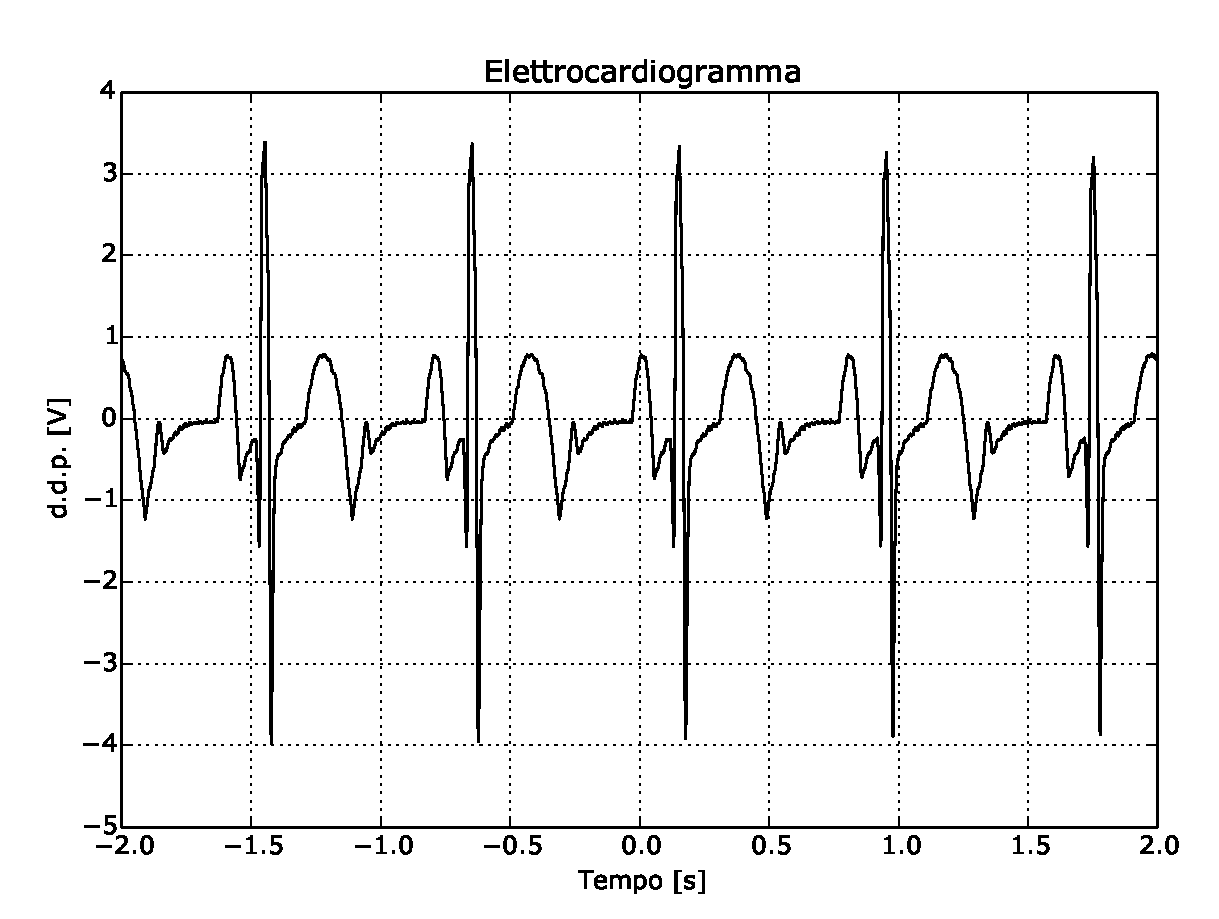
\includegraphics[height=0.32\textheight]{figure/ecg.pdf}
    \caption{Esempio di elettrocardiogramma misurato con il circuito che abbiamo montato.
        Il battito é di 75 battiti/minuto. Misurando la distanza tra i picchi,
        abbiamo notato che il cuore é estremamente preciso: ogni picco é distanziato da quello
        vicino da circa 800 ms, con una deviazione massima di 2 ms. Sono inoltre visibili altri
        picchi secondari, dovuti a varie fasi dell'attivitá cardiaca. Il paziente era uno dei
        membri del gruppo.}
    \label{fig:ecg7}
\end{SCfigure*}

\begin{SCfigure*}[][p]
    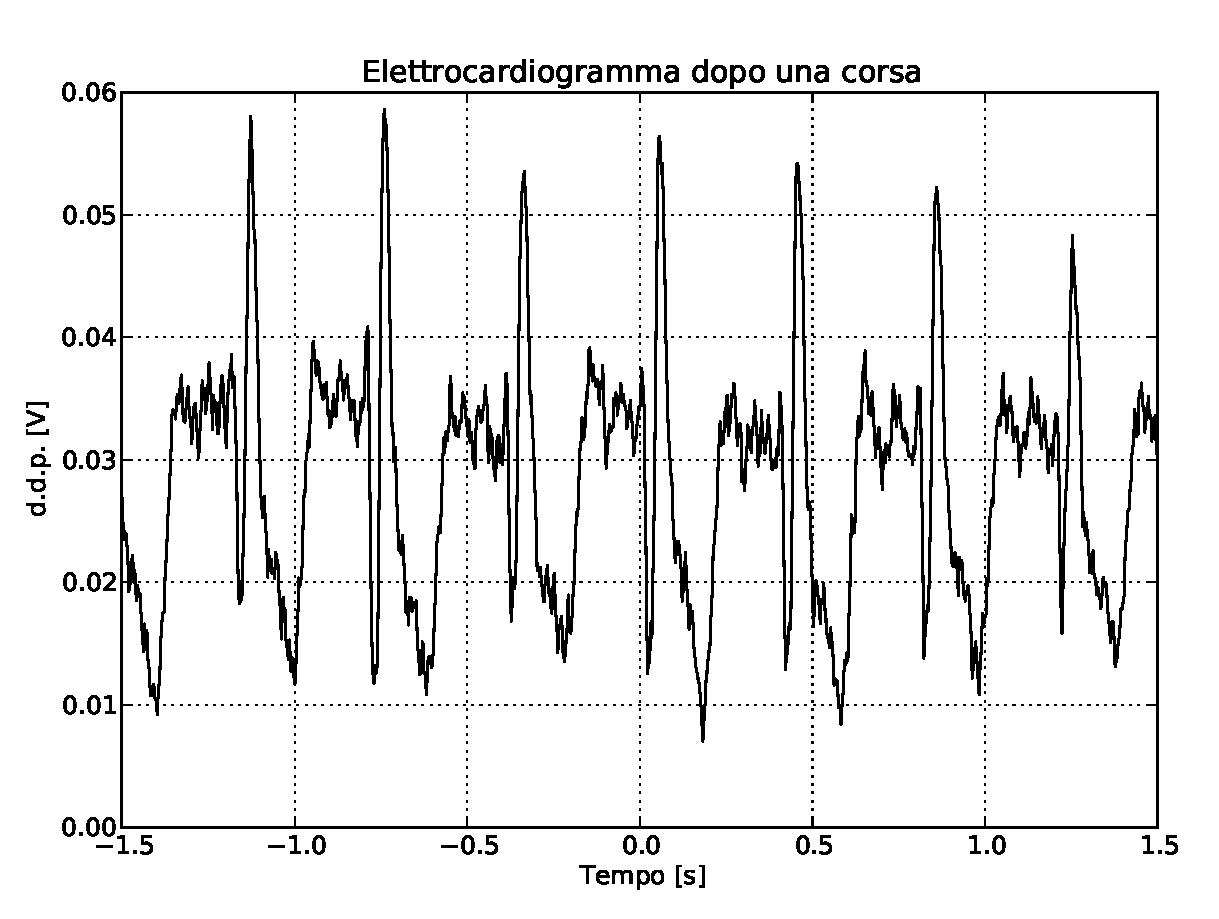
\includegraphics[height=0.32\textheight]{figure/ecg_corsa.pdf}
    \caption{ECG dello stesso soggetto dell'ECG in figura \ref{fig:ecg7} soltanto che in questo caso
        il paziente é uscito dal laboratorio e ha percorso qualche centinaio di metri di corsa prima della misura.
        Di conseguenza, il battito é salito a circa 150 battiti/minuto, o circa 400 ms tra i battiti, sempre con una
        precisione di pochi millisecondi. Questo ECG é un poco piú rumoroso del precedente.}
    \label{fig:ecg_corsa7}
\end{SCfigure*}

Dopo aver montato il circuito, ne abbiamo testato il comportamento provando a misurare l'elettrocardiogramma
di uno dei membri del gruppo. Il risultato è stato molto incoraggiante. In figura \ref{fig:ecg7} è mostrata
la registrazione ottenuta. Si possono notare le varie fasi dell'attività cardiaca, che approfondiremo nel
prossimo paragrafo. Inoltre si nota che la frequenza è circa 75 battiti/minuto, un valore tipico.
In figura \ref{fig:ecg_corsa7} vediamo invece un elettrocardiogramma fatto dopo che lo stesso soggetto
era uscito per compiere qualche centinaio di metri di corsa. Il battito cardiaco è ora attorno a 150 battiti/minuto!

\begin{SCfigure*}[][p]
    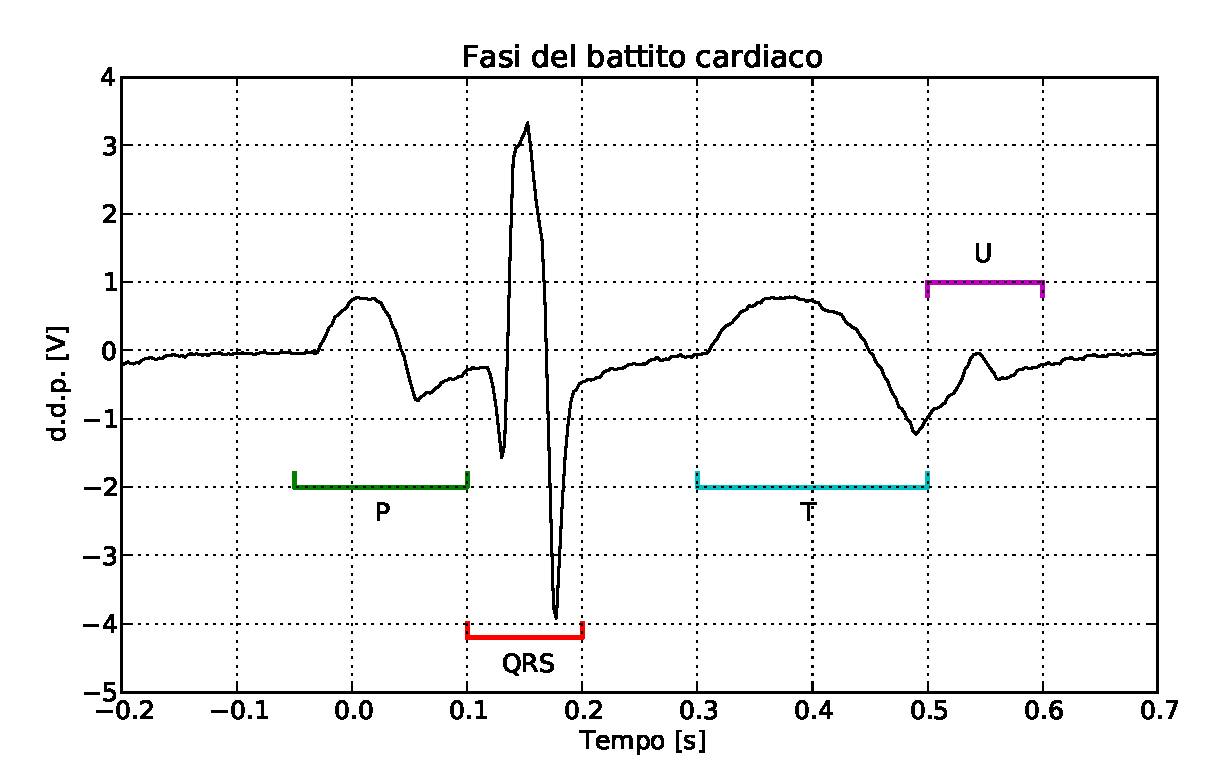
\includegraphics[height=0.32\textheight]{figure/ecg_fasi.pdf}
    \caption{Quest'immagine é un ingrandimento della figura \ref{fig:ecg7} e rappresentano un tipico
        battito cardiaco visto tramite ECG. Si vedono molto bene le varie onde generate dalle fasi dell'attivitá cardiaca.
        Riassumendo quanto scritto nel testo: \textbf{P} é la fase di contrazione degli atrii, \textbf{QRS} é l'onda generata dalla
        contrazione dei ventricoli, \textbf{T} é il rilassamento dei ventricoli e \textbf{U} é generata dal setto interventricolare.}
    \label{fig:ecg_fasi7}
\end{SCfigure*}

Un'analisi piú dettagliata dell'ECG fa riferimento alla figura \ref{fig:ecg_fasi7}.
In questa immagine é mostrato uno spezzone ingrandito dell'ECG della figura \ref{fig:ecg7}.
Sono distinguibili diverse fasi dell'attivitá cardiaca:

\begin{itemize}
    \item{Onda P: É dovuta alla depolarizzazione degli atrii, ovvero alla loro contrazione. In questa fase il sangue viene
        pompato dagli atrii ai ventricoli.}
    \item{Complesso QRS: É dovuto alla contrazione dei ventricoli, ovvero alla fase durante la quale il sangue viene pompato
        fuori dal cuore. Poiché i ventricoli hanno una massa muscolare molto maggiore a quella degli atrii, il picco é molto piú
        pronunciato.}
    \item{Onda T: In questa fase i ventricoli si ripolarizzano, ovvero si rilassano, risucchiando sangue dall'esterno.}
    \item{Onda U: Non é ben chiaro a cosa sia dovuta. L'ipotesi piú plausibile é che rappresenti la ripolarizzazione del
        setto interventricolare. Spesso é assente. Tuttavia nel caso in cui fosse troppo prominente, é un sintomo di alcune malattie cardiache.}
\end{itemize}
